\announcesection{Data Processing}

% Tracks
\frame{
    \frametitle{Tracking}
    \begin{columns} \begin{column}{0.5\textwidth}
    {\footnotesize
        2T solenoid magnet bends charged particles traversing trackers.
        Helical trajectory is used to calculated particle momentum/mass/charge.
    }
    \vspace{5mm}

    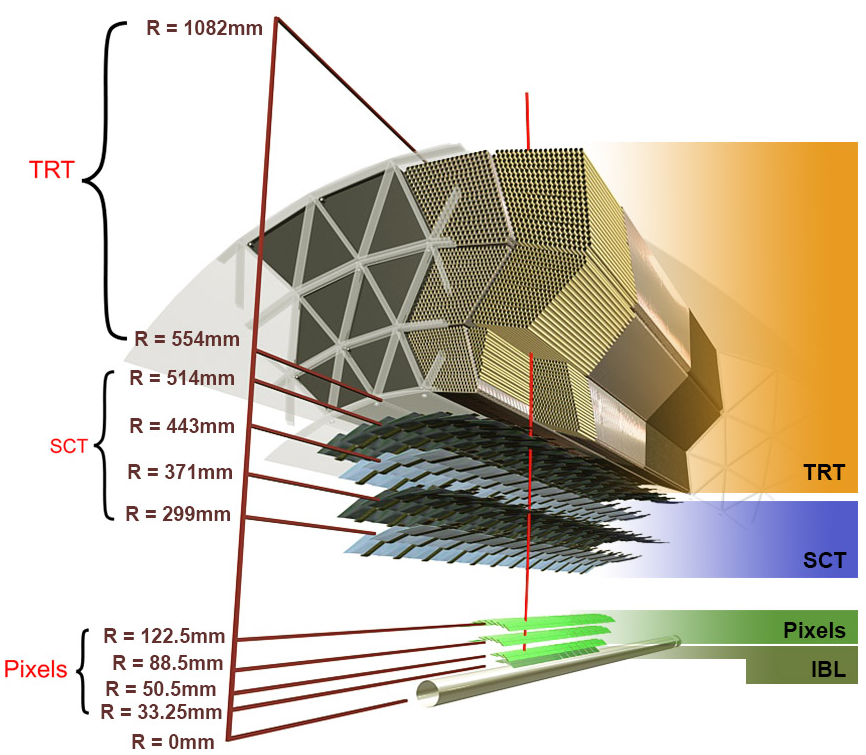
\includegraphics[width=\linewidth,height=0.9\textheight,keepaspectratio]{atlas/inner_detector_barrel_measurements}
    \end{column} \begin{column}{0.5\textwidth}
    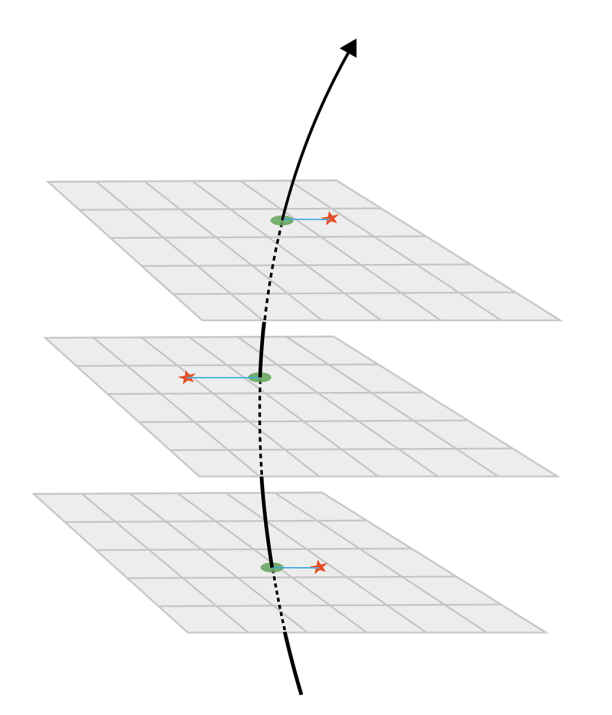
\includegraphics[width=\linewidth,height=0.9\textheight,keepaspectratio]{processing/tracking_hits}
    \end{column} \end{columns}
}

\displayonelarge{Calorimetry}{
    {\footnotesize
        Determines energy of particles by seeing how many plates of metal they can go through.
        E-Cal for electrons/photons,
            H-Cal for hadronic particles.

    }
}{reconstruction/ATLAS_Detector_Schematic_black_particles}

\frame{
    \frametitle{Jets}
    { \footnotesize
    Calorimeter clusters are grouped together and, if possible,
        associated with tracks to produce a complete picture of a particle's travel through ATLAS,
        forming an object called a ``jet.''
    }
    \vspace{5mm}

    \begin{columns} \begin{column}{0.24\textwidth}
    { \tiny
        Using anti-$k_t$(R=0.4) ``sequential recombination'' algorithm:

        \begin{equation} \begin{split}
            d_{ij} &= \textrm{min}(k_{ti}^{-2},k_{tj}^{-2}) \frac{\Delta_{ij}^2}{R^2}; \\
            d_{iB} &= k_{ti}^{-2};
            \nonumber
        \end{split} \end{equation}

        \begin{equation} \begin{split}
            &\textrm{if } d_{iB} \textrm{ is min:}\\
            &\qquad i=\textrm{jet;}\\
            &\qquad \textrm{remove jet;}\\
            &\textrm{else:}\\
            &\qquad \textrm{recombine min } i,j
            \nonumber
        \end{split} \end{equation}
    }

    \end{column} \begin{column}{0.75\textwidth}
    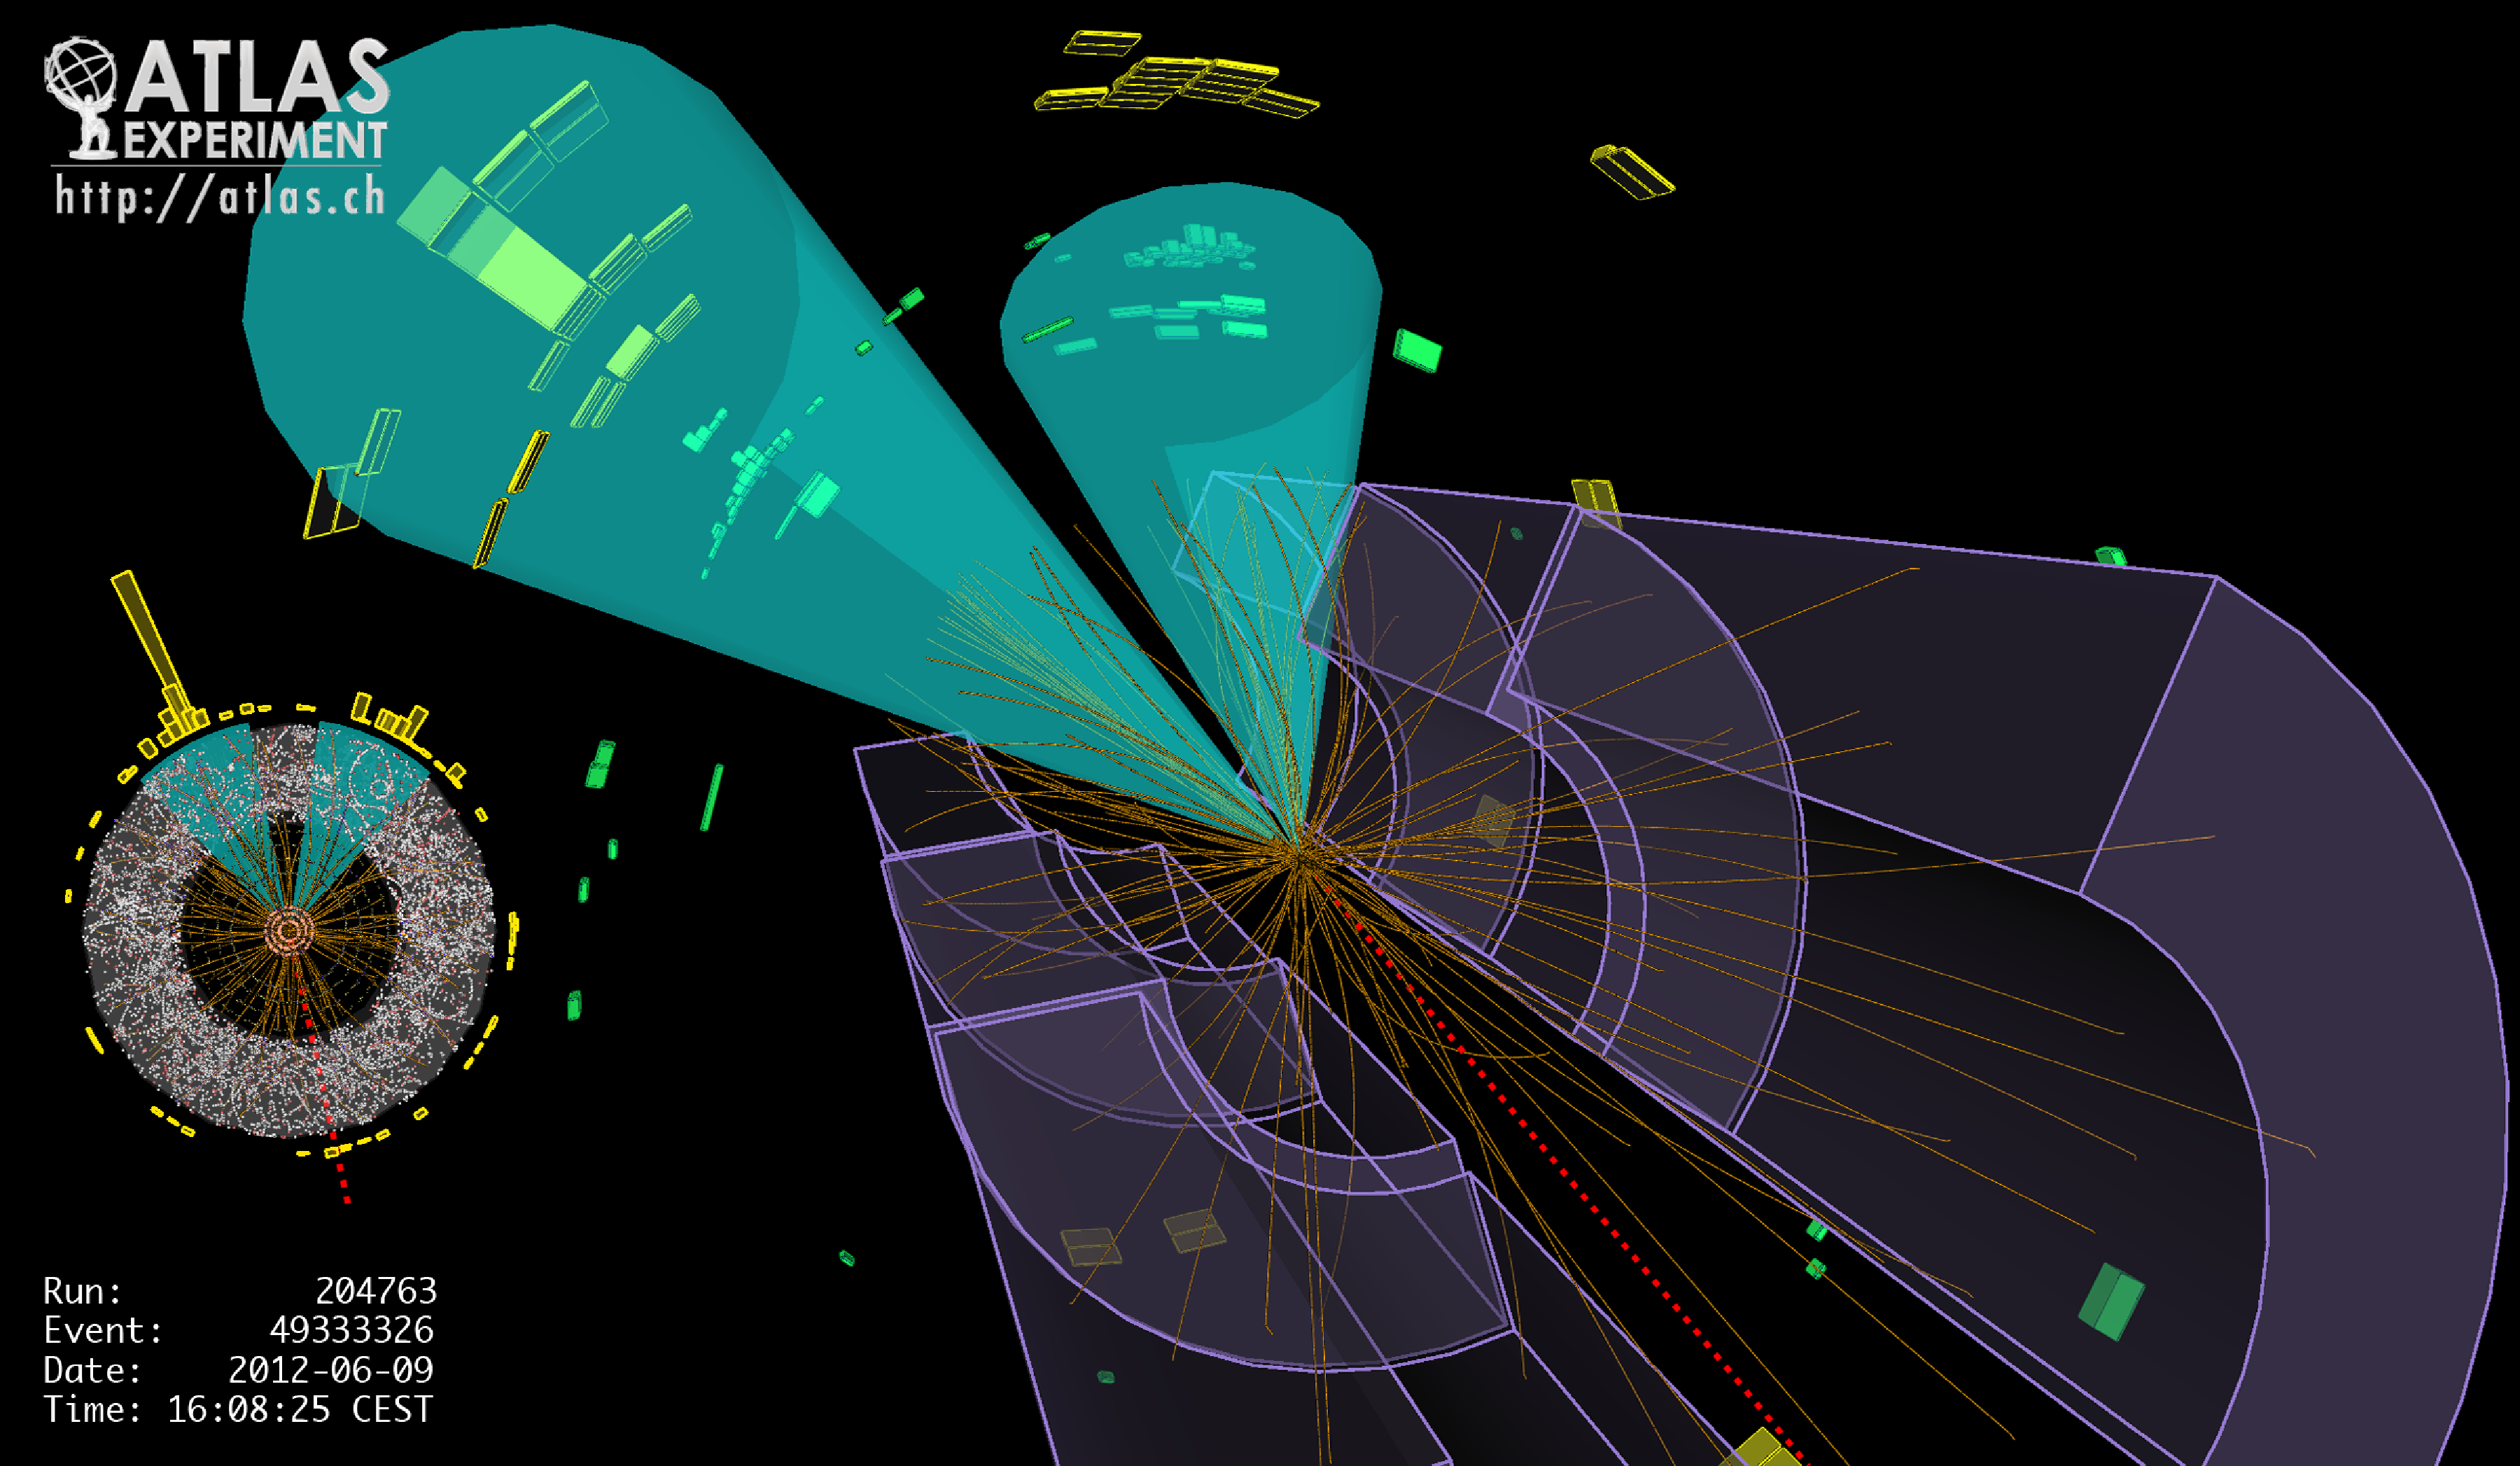
\includegraphics[width=\linewidth,height=\textheight,keepaspectratio]{processing/jets}
    \end{column} \end{columns}
}

\frame{
    \frametitle{Flavor Tagging}
    {\small Uses a Deep Learning neural net (DL1r@77\% working point) to distinguish b-jets from light-jets.
    Primarily takes advantage of secondary vertexing and impact parameter jet properties.}

    \begin{columns} \begin{column}{0.4\textwidth}
        \begin{figure}
            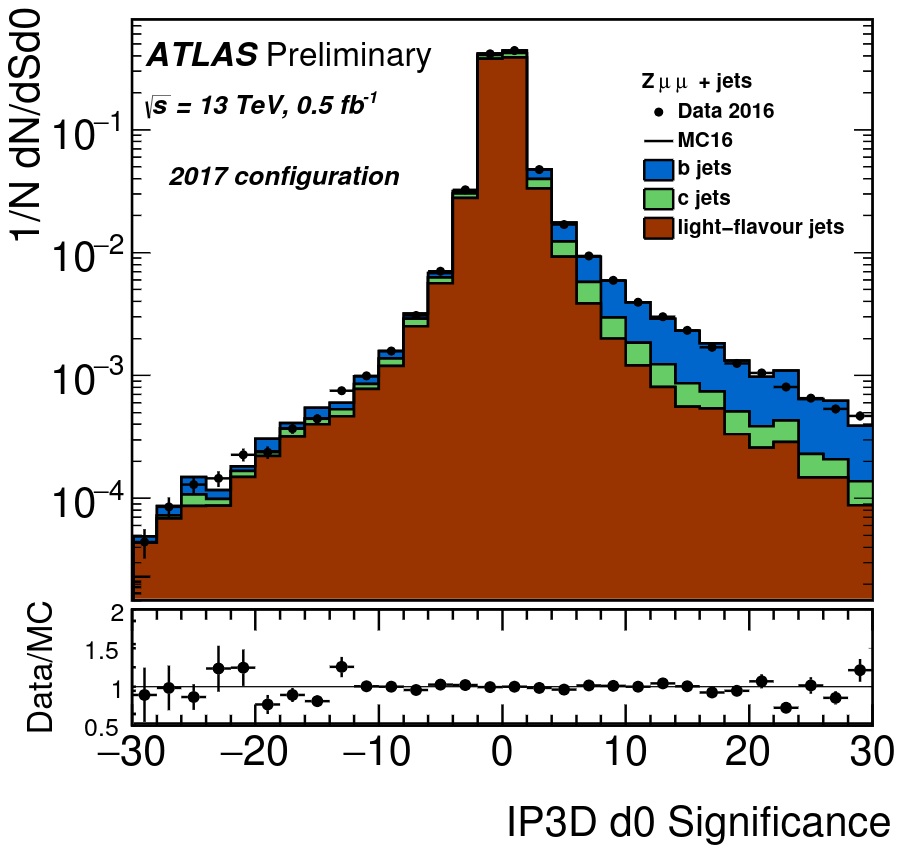
\includegraphics[width=\linewidth,height=\textheight,keepaspectratio]{reconstruction/ip3d_d0_sig_2017}
        \end{figure}
    \end{column} \begin{column}{0.6\textwidth}
    \begin{figure}
        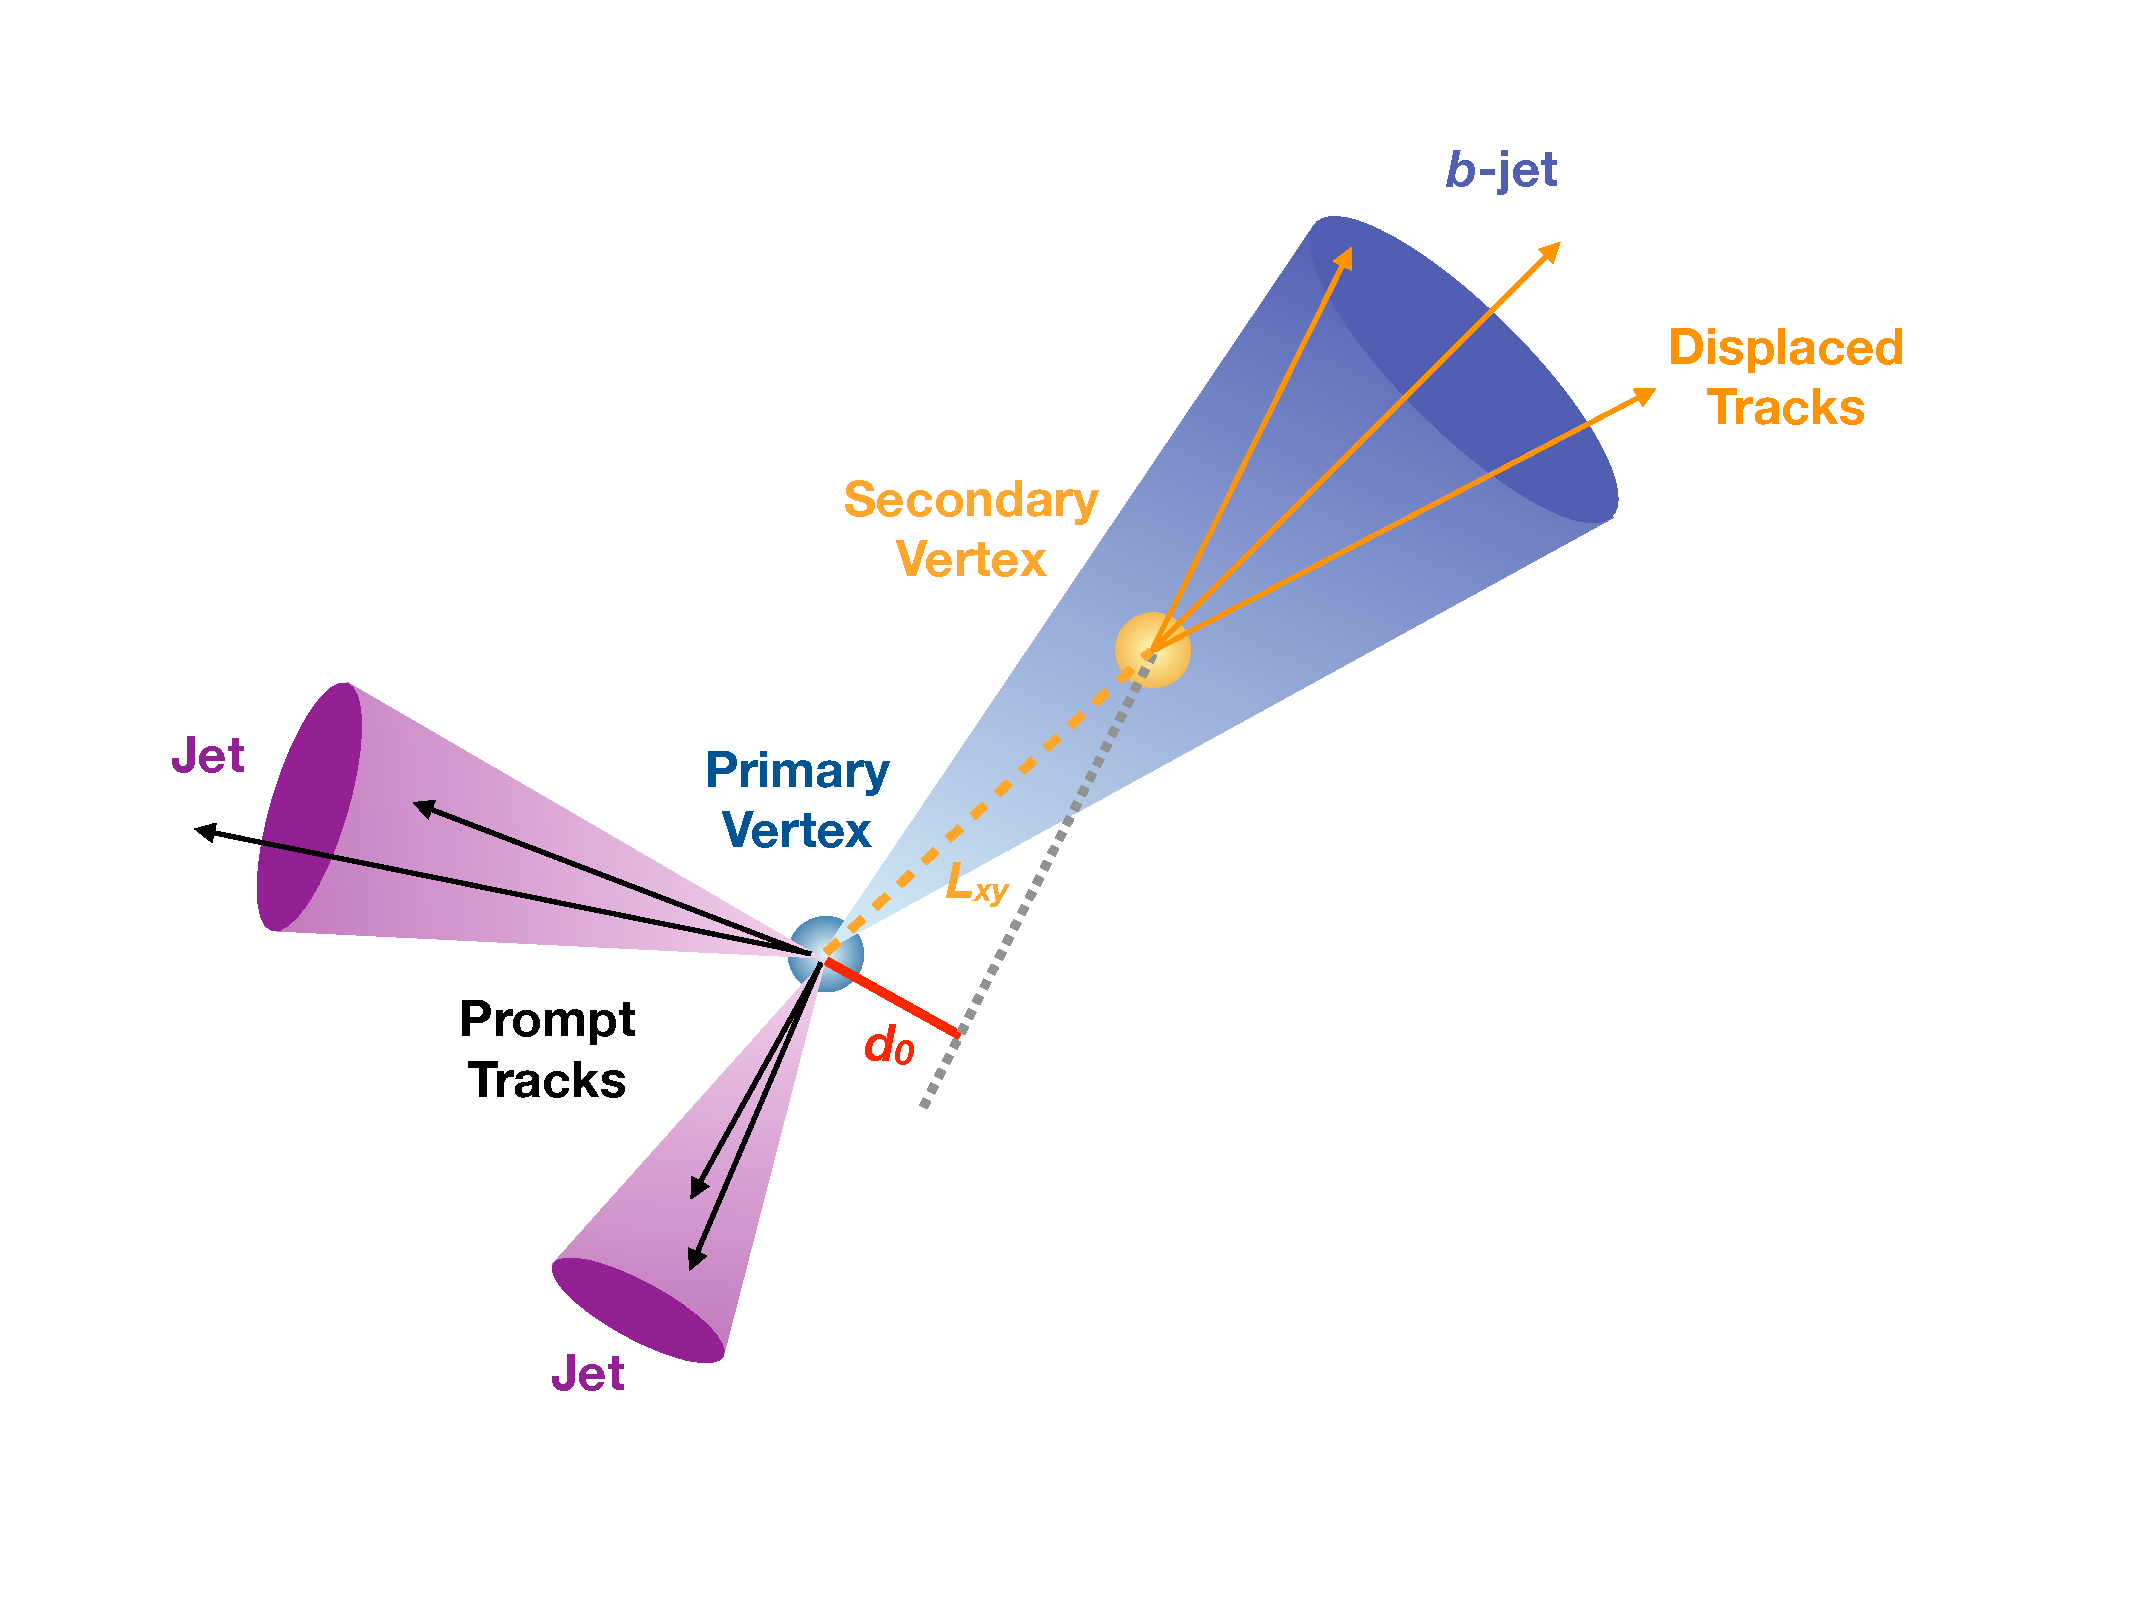
\includegraphics[width=\linewidth,height=\textheight,keepaspectratio]{processing/jet_vertexing}
    \end{figure}
    \end{column} \end{columns}
}


% Selection
\frame{
    \frametitle{Event Selection}
    \begin{columns} \begin{column}{0.39\textwidth}
        \begin{figure}
            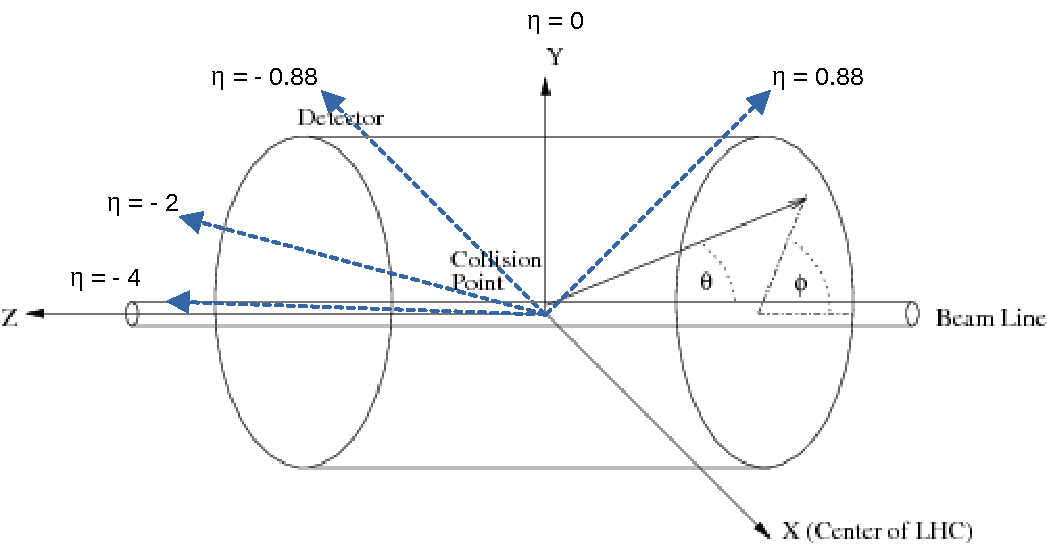
\includegraphics[width=\linewidth,height=0.3\textheight,keepaspectratio]{atlas/atlas_coords}
            \captionsetup{justification=centering}
            \caption*{ \tiny
                $\eta \equiv -\ln[\tan(\frac{\theta}{2})]$\\
                e.g. $\eta = .88 \to \theta=45^{\circ}$,\\$\eta = 4 \to \theta=2^{\circ}$
            }
        \end{figure}
        \vspace{-3mm}

        \resizebox{0.3\textheight}{!}{\vbox{
        \begin{itemize}
            \item At least six jets total
            \begin{itemize}
                \item Central Jets: $|\eta| < 2.5$, $p_T > 40$ GeV
                \item Forward Jets: $2.5 < |\eta| \leq 4.5$, $p_T > 30$ GeV
            \end{itemize}
            \item Two \textit{anti}-b-tagged jets
            \begin{itemize}
                \item $ |\Delta \eta_{jj}| > 3.0 $,
                \item $M_{jj} > 1000$ GeV, and
                \item $p_{T,jj} < 65 $ GeV
            \end{itemize}
            \item At least 4 central, b-tagged jets
            \begin{itemize}
                \item $p_T > 40$ GeV
                \item paired up as reconstructed HH
                \item $ |\Delta \eta_{HH}| < 1.5 $
            \end{itemize}
            \item Using b-jet trigger DL1r 77\% working point,
                light jet acceptance of 0.59\%
        \end{itemize}
        }}
    \end{column} \begin{column}{0.6\textwidth}
        \begin{figure}
            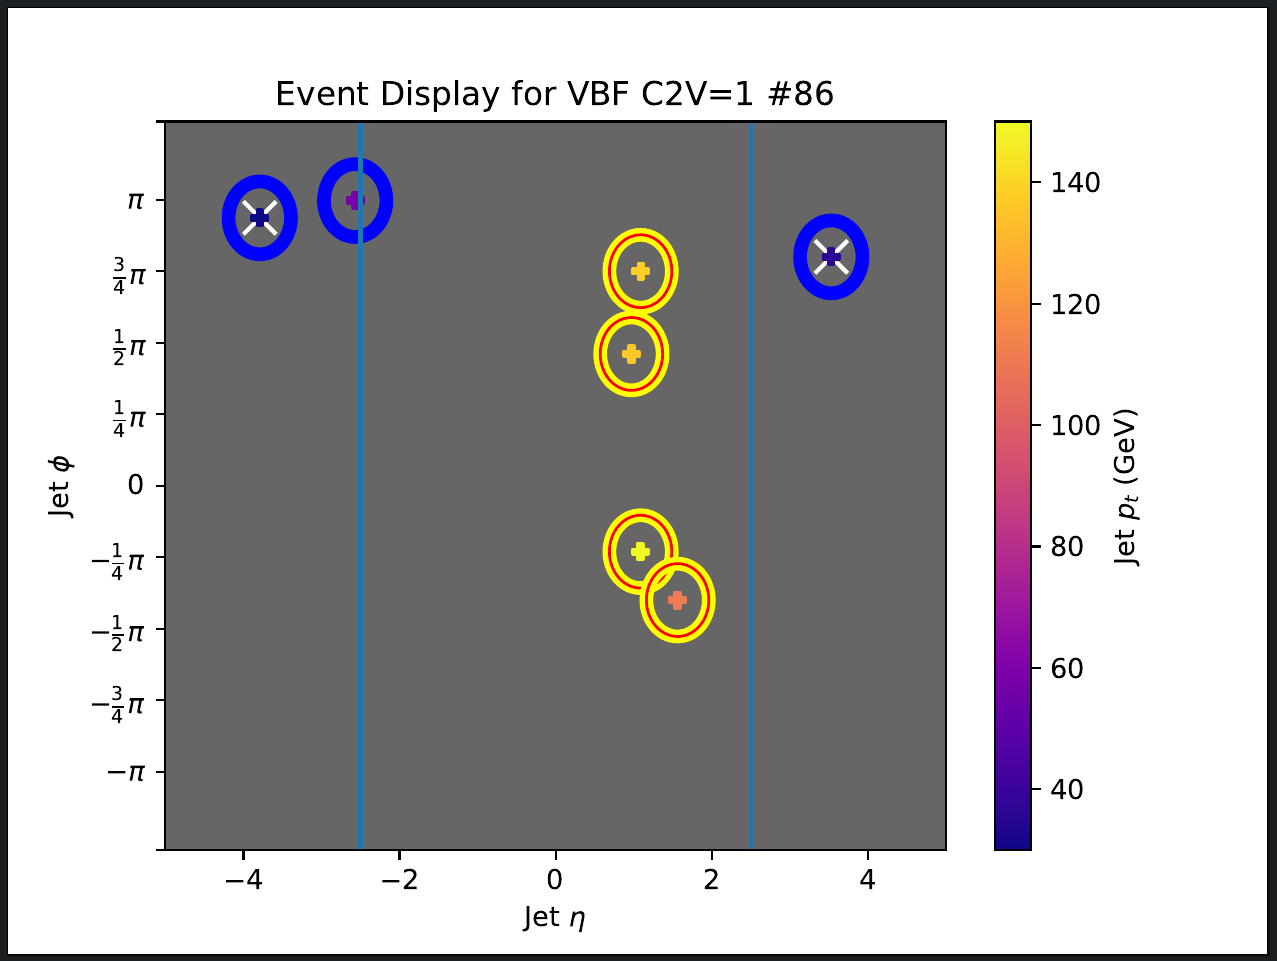
\includegraphics[width=\linewidth,height=0.5\textheight,keepaspectratio]{selection/event_display}
            \caption*{\tiny Rings indicate jets;
                Yellow ring => b-tagged;
                Blue ring w/ white cross => VBF initial-scatter jets;
                ``+'' in center of rings => $p_T$;
                vertical lines denote "forward" vs "central" region.}
        \end{figure}
    \end{column} \end{columns}
}

% Background Events
\frame{
    \frametitle{Massplane and Background Modelling}
    Multi-jet events (and some $\ttbar$) are a massive background.
    \vspace{3mm}

    Unlike the signal, the multi-jet background cannot be simulated through MC
    \begin{columns} \begin{column}{0.3\textwidth}
        {\footnotesize 
            MC simulated signal, massplane distribution
        }
    \end{column} \begin{column}{0.7\textwidth}
        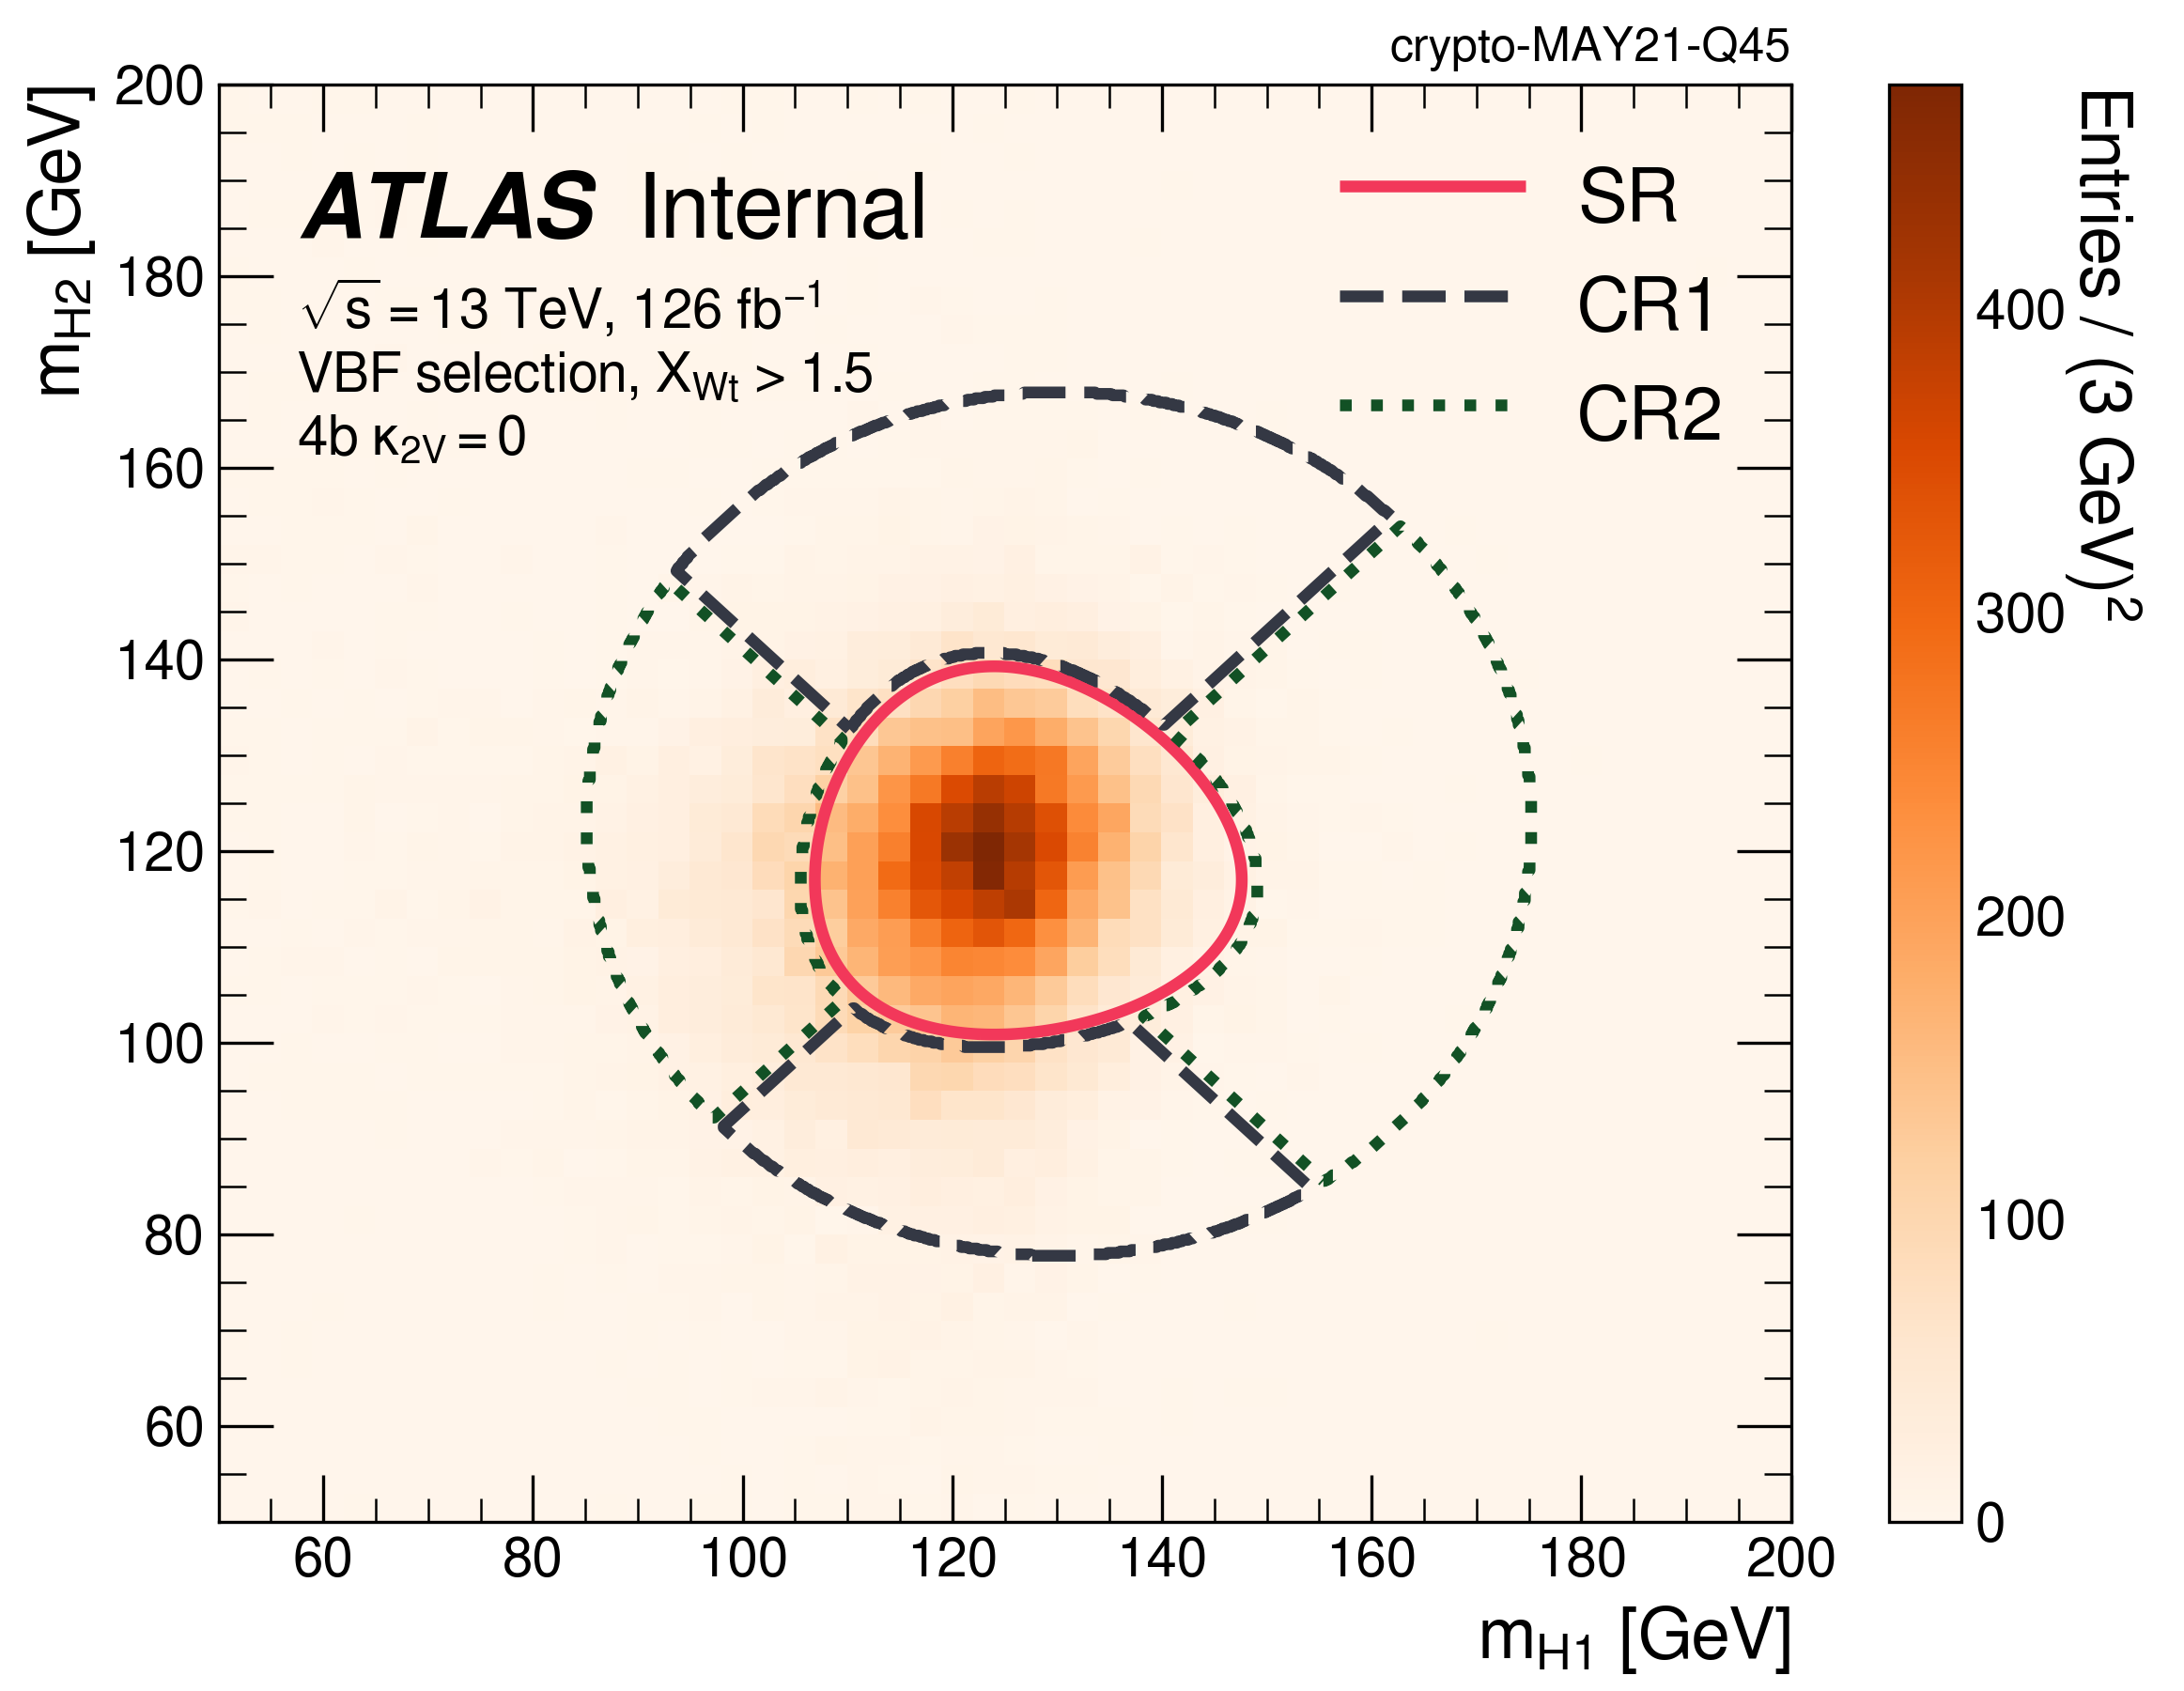
\includegraphics[width=\linewidth,height=0.9\textheight,keepaspectratio]
        {selection/massplane_sig_all_4b_vbf_Xwt_1p5_k2V_0}
    \end{column} \end{columns}
}

\displaytwocaption{Background in Control Regions}{
    Background is known outside signal region,
        because the data \textit{is} the background
        (no signal there).
}{selection/massplane_sig_all_4b_vbf_Xwt_1p5_k2V_0}
{MC simulated signal}
{background/massplane_dat_all_4b_vbf_Xwt_1.5}
{4b data sans signal region}

\displaytwocaption{Background in 2b Regions}{
    Likewise, background is known \textit{everywhere} in 2b data.
}
{background/massplane_dat_all_4b_vbf_Xwt_1.5}
{4b data sans signal region}
{background/massplane_dat_all_2b_vbf_Xwt_1.5}
{2b data}

\newcommand{\regt}[1]{
    \textrm{\footnotesize #1}
}
\frame{
    \frametitle{Data-driven Background Estimate}
    Background hypothesized to be kinematically indifferent to number of b-jets.
    \vspace{3mm}

    Thus, combining the 2b data with the 4b control region
        allows estimate of background in 4b signal region.

    \begin{figure}
        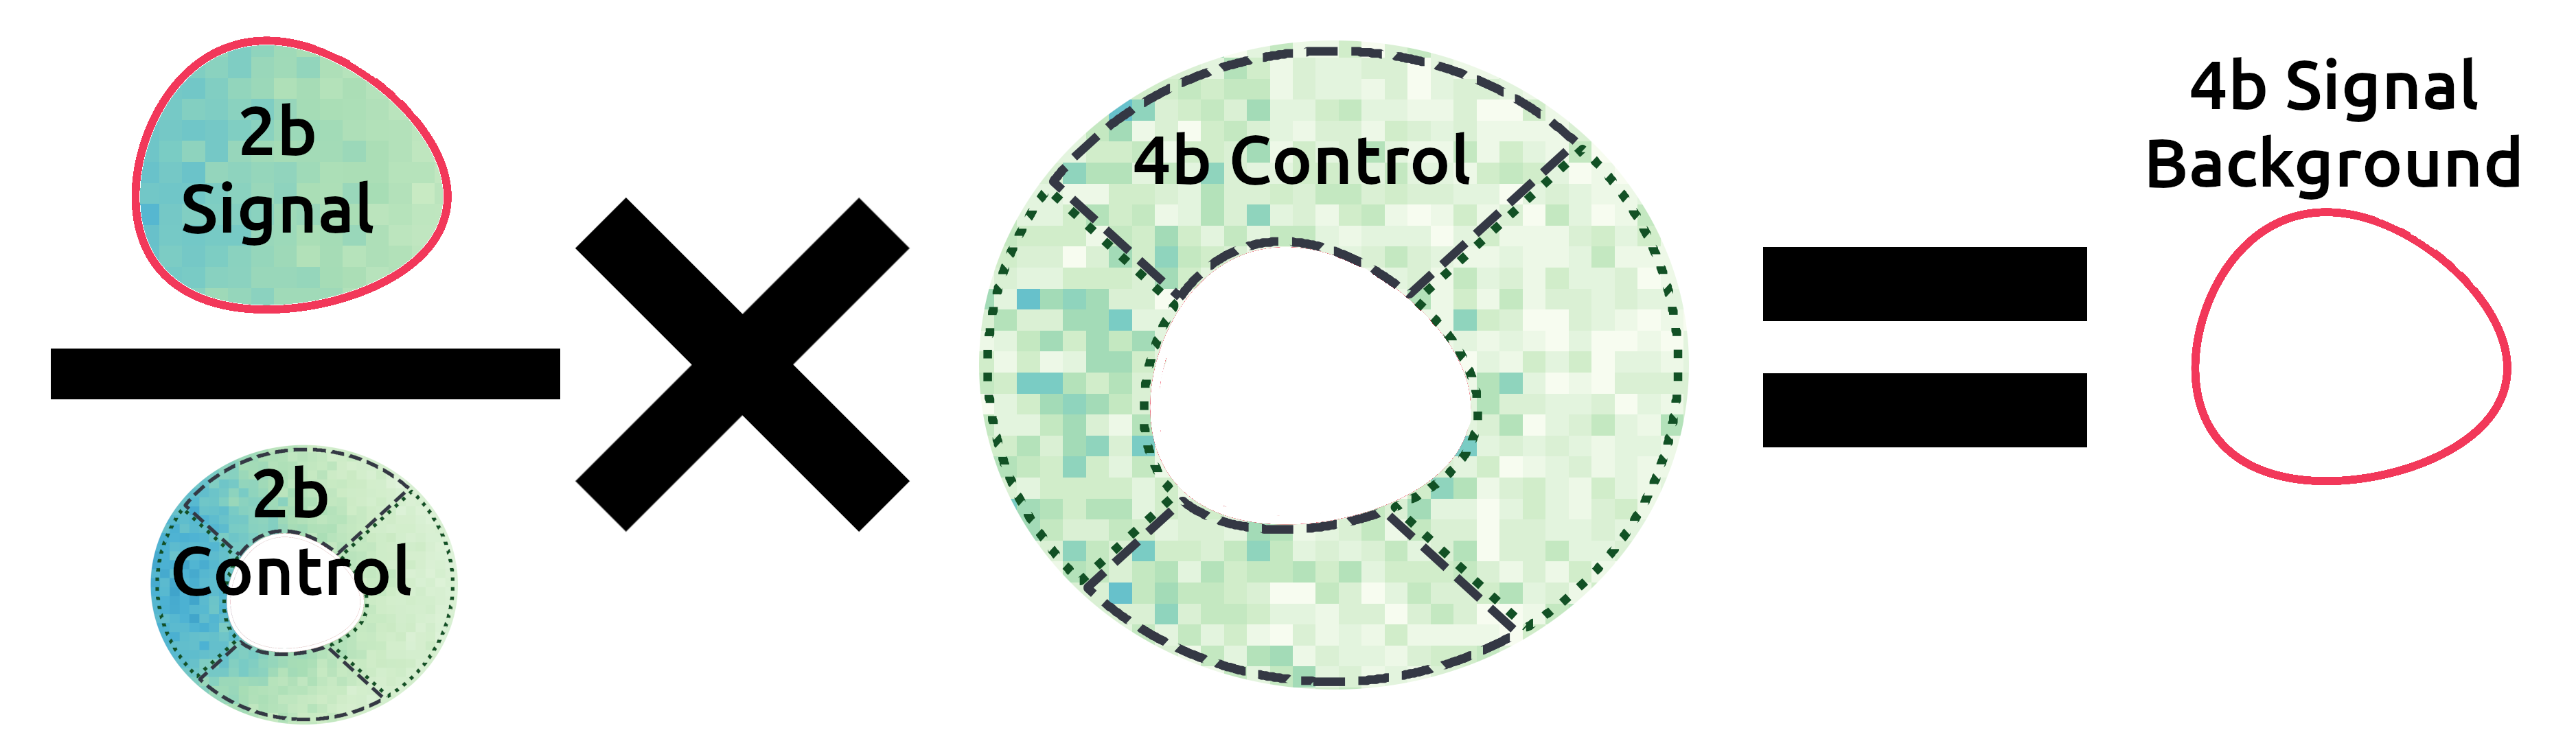
\includegraphics[width=\linewidth,keepaspectratio]
        {processing/bgd_rw_eq}
    \end{figure}
    \vspace{5mm}

    \begin{center} {\Huge
        $ \frac{58,731\regt{2b sig} }{110,843\regt{2b control} }
        \times
        947 \regt{4b control}
        =
        502 \regt{4b sig} $
    } \end{center}
}


%\displaytwo{Data-driven Background Estimate}{
%    \footnotesize{
%        Multi-jet events (and some $\ttbar$ events) are a massive background.
%
%        But unlike the signal, the multi-jet background cannot be simulated through MC
%
%        %Can use data in which only 2 jets are b-tagged
%        %    and massplane ``control regions'' to estimate background present in signal region.
%    }
%    \vspace{5mm}
%
%    \begin{center}
%    $ \textrm{Bgd}(4b, \textrm{Signal}) \approx 
%         \textrm{Bgd}(4b, \textrm{Control}) \times \frac{
%         \textrm{Bgd}(2b, \textrm{Signal}) }{
%         \textrm{Bgd}(2b, \textrm{Control})} $
%     \end{center}
%    
%    %Posit that 2b-tagged events are kinematically similar to 4b-tagged background.
%
%}{selection/massplane_sig_all_4b_vbf_Xwt_1p5_k2V_0}
%{background/massplane_dat_all_2b_vbf_Xwt_1.5}

\displayone{Background Reweighting}{
    {\footnotesize
        Kinematic differences exist between 2b and 4b;
             requires event-by-event reweighting

        \begin{center} 
        Example event:
        \vspace{3mm}

        \resizebox{0.3\textheight}{!}{ \begin{tabular}{ |l|r| }
            \hline
                $p_{T,H1}$ & 80 GeV \\ \hline
                $p_{T,H2}$ & 75 GeV \\ \hline
                $m_{HH}$ & 500 GeV \\ \hline
                $m_{jj}$ & 1200 GeV \\ \hline
                $\deta_{HH}$ & 1.1 \\ \hline
                \textbf{2b} rate & 8\% \\ \hline
                \textbf{4b} rate & 5\% \\ \hline
        \end{tabular}}
        \vspace{5mm}

            $\therefore$ reweight such an event by factor of 5/8
        \end{center}
        \vspace{3mm}
    }
}{background/NR-UNBLIND-FEB22-2-m-hh-Control-Region-1-no-rw-all-4binclusive}

\displayfourCcaption{Reweighting Performance}
{{\tiny Before reweighting\vspace{2mm}}}
{{\tiny After reweighting\\\vspace{-2mm}(Note: ``Stat. Error'' here is stat+sys)}}
{background/NR-UNBLIND-FEB22-2-m-hh-Control-Region-1-no-rw-all-4binclusive}
{background/NR-UNBLIND-FEB22-2-m-hh-Control-Region-1-NN-all-4binclusive}
{background/NR-UNBLIND-FEB22-2-dEta-hh-Control-Region-1-no-rw-all-4binclusive}
{background/NR-UNBLIND-FEB22-2-dEta-hh-Control-Region-1-NN-all-4binclusive}

%{background/crypto-mean-stdBS-X-wt-tag-Control-Region-1-no-rw-all-4binclusive}
%{background/crypto-mean-stdBS-X-wt-tag-Control-Region-1-NN-all-4binclusive}
